\question {
    现有一个长度为$5$的整数数组,假设需要写一个两线程程序,其中,线程$1$负责往数组中写入$5$个随机数($1$到$20$范围内的随机整数),写完这$5$个数后,线程$2$负责从数组中读取这$5$个数,并求和。该过程循环执行$5$次。注意:每次循环开始时,线程1都重新写入$5$个数。请思考:
}
\begin{enumerate}
    \item 上述过程能否通过{\tt pthread_mutex_lock/unlock()}函数实现?如果可以,请写出相应的源代码,并运行程序,打印出每次循环计算的求和值;如果无法实现,请分析并说明原因。
\end{enumerate}

提交:

实现题述功能的源代码和打印结果,或者无法实现的原因分析说明。

\begin{solution}

源代码如下:
\lstinputlisting[language=C]{code/2.c}

打印结果如下:
\begin{figure}[H]
    \centering
    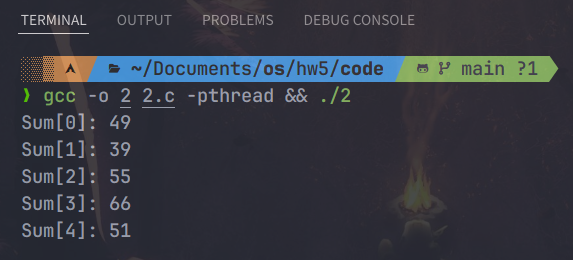
\includegraphics[width=0.6\textwidth]{img/2.png}
    \caption{打印结果}
\end{figure}

\end{solution}
